% Build: module load texlive/20240312-GCC-13.3.0 && pdflatex top.tex (twice)
% Simplified deck built around diagrams. The detailed version is top_v1.tex.
% Facts: /nfs/roberts/scratch/pi_nrs36/jar335/rebuild/explore/2026-10-29/top_build/{hidden,billionaires}/RESULTS.md

% Shared look, copied from ../2026-10_rebuild/rebuild_talk.tex (lines 1-75)

\documentclass[11pt,aspectratio=169]{beamer}

% ---------------------------------------------------------------------------
% Look: plain beamer, Yale colours
% ---------------------------------------------------------------------------
\usetheme{default}
\usefonttheme{professionalfonts}
\setbeamertemplate{navigation symbols}{}

\definecolor{yaleblue}{HTML}{00356B}
\definecolor{yalemid}{HTML}{286DC0}
\definecolor{yalelight}{HTML}{63AAFF}
\definecolor{yalegrey}{HTML}{4A4A4A}
\definecolor{yalelightgrey}{HTML}{DDDDDD}

\setbeamercolor{structure}{fg=yaleblue}
\setbeamercolor{normal text}{fg=black}
\setbeamercolor{frametitle}{fg=yaleblue}
\setbeamercolor{title}{fg=yaleblue}
\setbeamercolor{alerted text}{fg=yalemid}
\setbeamercolor{block title}{fg=white,bg=yaleblue}
\setbeamercolor{block body}{bg=yalelightgrey!40}

\setbeamerfont{frametitle}{series=\bfseries,size=\large}
\setbeamerfont{title}{series=\bfseries,size=\Large}

\setbeamertemplate{itemize items}[circle]
\setbeamertemplate{blocks}[rounded][shadow=false]

% A thin blue rule under each frame title
\setbeamertemplate{frametitle}{%
  \vspace*{0.6em}%
  \usebeamerfont{frametitle}\usebeamercolor[fg]{frametitle}\insertframetitle\par
  \vspace*{-0.2em}{\color{yaleblue}\rule{\textwidth}{0.6pt}}%
}

% Footer: short title on the left, slide number on the right
\setbeamertemplate{footline}{%
  \hspace*{1.2em}{\color{yalegrey}\scriptsize\insertshorttitle}%
  \hfill{\color{yalegrey}\scriptsize\insertframenumber}\hspace*{1.2em}%
  \vspace*{0.6em}%
}

% ---------------------------------------------------------------------------
% Packages
% ---------------------------------------------------------------------------
\usepackage[T1]{fontenc}
\usepackage{lmodern}
\usepackage{booktabs}
\usepackage{array}
\usepackage{graphicx}
\usepackage{amsmath}
\usepackage{tikz}
\usetikzlibrary{positioning,arrows.meta,calc}
\usepackage{pgfplots}
\pgfplotsset{compat=1.18}
\graphicspath{{figures/}}

% Diagram styles
\tikzset{
  tok/.style={draw=yaleblue, rounded corners=2pt, font=\small, inner sep=4pt,
              minimum height=0.65cm},
  blank/.style={tok, fill=yalelight!35, font=\small\bfseries},
  box/.style={draw=yaleblue, rounded corners=2pt, font=\scriptsize, align=center,
               text width=2.1cm, minimum height=1.1cm, inner sep=3pt},
  arr/.style={-{Stealth[length=5pt]}, yaleblue, thick},
  cF/.style={fill=yaleblue},
  cP/.style={fill=yalelight!60},
  cN/.style={fill=white},
}

\pgfplotsset{colormap={yalemap}{color=(white) color=(yalelight) color=(yaleblue)}}



\tikzset{
  nb/.style={draw=yaleblue, rounded corners=3pt, align=center, font=\small,
             inner sep=5pt, minimum height=0.9cm, fill=white},
  old/.style={nb, fill=yalelightgrey!60},
  new/.style={nb, fill=yalelight!35, line width=1pt},
  sm/.style={nb, font=\footnotesize, inner sep=3pt, minimum height=0.55cm},
  note/.style={draw=yalegrey, dashed, rounded corners=3pt, align=left,
               font=\footnotesize, inner sep=5pt, text width=4.6cm},
}

\title[Top of the file]{The PUF's aggregate records and the billionaires\\in the Tax-Data rebuild}
\author{John Ricco}
\institute{The Budget Lab at Yale}
\date{October 2026}

\hyphenpenalty=10000
\exhyphenpenalty=10000

\begin{document}

\begin{frame}[plain,noframenumbering]
  \titlepage
\end{frame}

% 2
\begin{frame}{The rebuild in one picture}
  \centering
  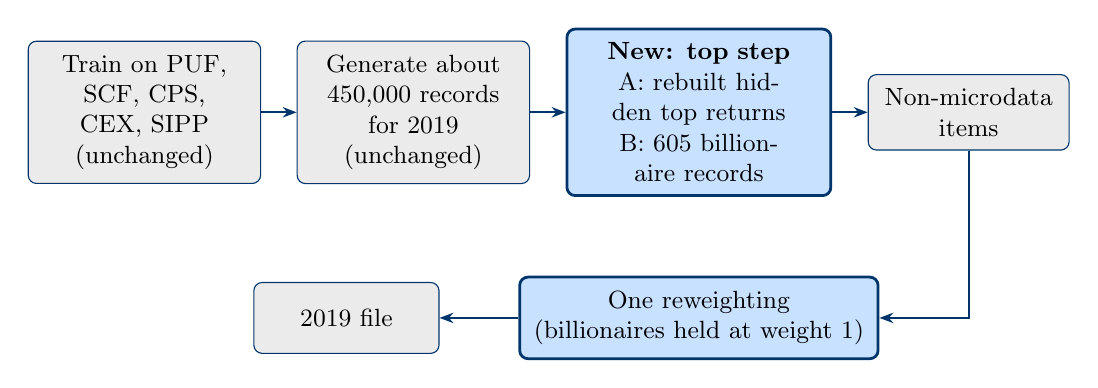
\begin{tikzpicture}[node distance=0.45cm]
    \node[old, text width=2.6cm] (a) {Train on PUF, SCF, CPS, CEX, SIPP\\(unchanged)};
    \node[old, text width=2.6cm, right=of a] (b) {Generate about 450,000 records for 2019\\(unchanged)};
    \node[new, text width=3.0cm, right=of b] (c) {\textbf{New: top step}\\A: rebuilt hidden top returns\\B: 605 billionaire records};
    \node[old, text width=2.2cm, right=of c] (d) {Non-microdata items};
    \draw[arr] (a)--(b); \draw[arr] (b)--(c); \draw[arr] (c)--(d);
    \node[new, text width=4.2cm, below=1.0cm of c] (e) {One reweighting\\(billionaires held at weight 1)};
    \node[old, text width=2cm, left=1.0cm of e] (f) {2019 file};
    \draw[arr] (d.south) |- (e.east);
    \draw[arr] (e.west)--(f.east);
  \end{tikzpicture}

  \vspace{1.2em}
  \small Two things change: about 2,800 records are added before the reweighting, and the
  billionaires' weights cannot move.
\end{frame}

% 3
\begin{frame}{Problem 1: the PUF's aggregate records}
  \small
  In the 2015 PUF, SOI folded 1,233 extreme returns into four records that hold group means.
  Together they hold \$140 billion of AGI.
  \vspace{0.5em}
  \begin{center}
    \begin{tabular}{lrr}
      \toprule
      AGI group & Returns & Total AGI \\
      \midrule
      Negative AGI        & 140 & $-$\$13.5bn \\
      \$0--10 million     & 233 & \$0.9bn \\
      \$10--100 million   & 394 & \$17.2bn \\
      Over \$100 million  & 465 & \$135.7bn \\
      \bottomrule
    \end{tabular}
  \end{center}
  \vspace{0.3em}
  The retained PUF cannot reach SOI's top 0.001\% by AGI: its largest AGI, \$136 million, is below
  that group's mean, \$152 million.
  \par\vfill{\scriptsize\color{yalegrey}2015 dollars.}
\end{frame}

% 4
\begin{frame}{Problem 2: the billionaires, and why not add them before training}
  \small
  The SCF drops the Forbes 400 by name. The PUF hides them in its aggregate records.
  \vspace{0.5em}

  Adding them to the training data would not work:
  \begin{itemize}
    \item A few hundred rows among about 136,000 SCF rows would barely move the network.
    \item The list gives wealth but no tax items to learn from.
    \item Drawn dollar amounts cannot exceed the training data's largest values.
  \end{itemize}
  \vspace{0.5em}
  So both problems are handled after generation, before the reweighting.
\end{frame}

% 5
\begin{frame}{Part A: rebuilding the aggregate records}
  \begin{columns}[c]
    \begin{column}{0.64\textwidth}
      \centering
      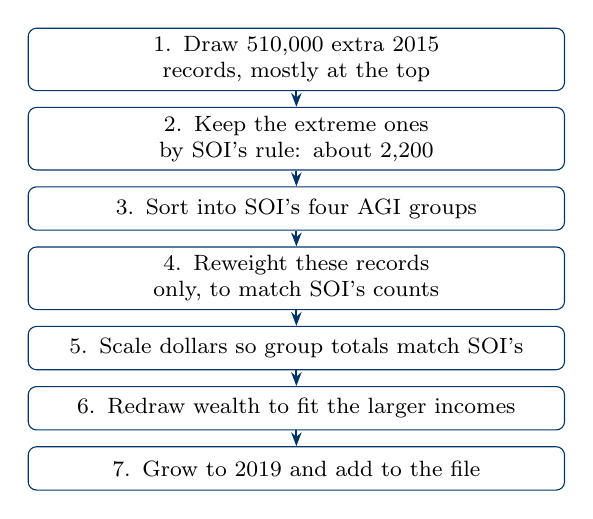
\begin{tikzpicture}[node distance=0.2cm]
        \node[sm, text width=6.6cm] (s1) {1. Draw 510,000 extra 2015 records, mostly at the top};
        \node[sm, text width=6.6cm, below=of s1] (s2) {2. Keep the extreme ones by SOI's rule: about 2,200};
        \node[sm, text width=6.6cm, below=of s2] (s3) {3. Sort into SOI's four AGI groups};
        \node[sm, text width=6.6cm, below=of s3] (s4) {4. Reweight these records only, to match SOI's counts};
        \node[sm, text width=6.6cm, below=of s4] (s5) {5. Scale dollars so group totals match SOI's};
        \node[sm, text width=6.6cm, below=of s5] (s6) {6. Redraw wealth to fit the larger incomes};
        \node[sm, text width=6.6cm, below=of s6] (s7) {7. Grow to 2019 and add to the file};
        \foreach \i/\j in {1/2,2/3,3/4,4/5,5/6,6/7} \draw[arr] (s\i)--(s\j);
      \end{tikzpicture}
    \end{column}
    \begin{column}{0.34\textwidth}
      \footnotesize
      The network supplies which items go together. SOI's published totals supply the sizes.

      \vspace{0.6em}
      The method follows Ricco (2020) for the Penn Wharton Budget Model.
    \end{column}
  \end{columns}
\end{frame}

% 6
\begin{frame}{Part A: a worked example}
  \small
  Illustrative numbers.
  \vspace{0.4em}
  \begin{enumerate}
    \item \textbf{Weights.} SOI's over-\$100-million record stands for 465 returns. We keep 600
          records, so each starts at 465/600 = 0.775. The weights are then nudged until SOI's counts match.
    \item \textbf{Dollars.} SOI's group total of long-term gains is \$80 billion. Our weighted records
          total \$30 billion. Every record's gains in that group are multiplied by 80/30 = 2.67.
    \item Gains and losses are scaled separately. AGI is recomputed from the parts.
  \end{enumerate}
\end{frame}

% 7
\begin{frame}{Part B: building the billionaire records}
  \centering
  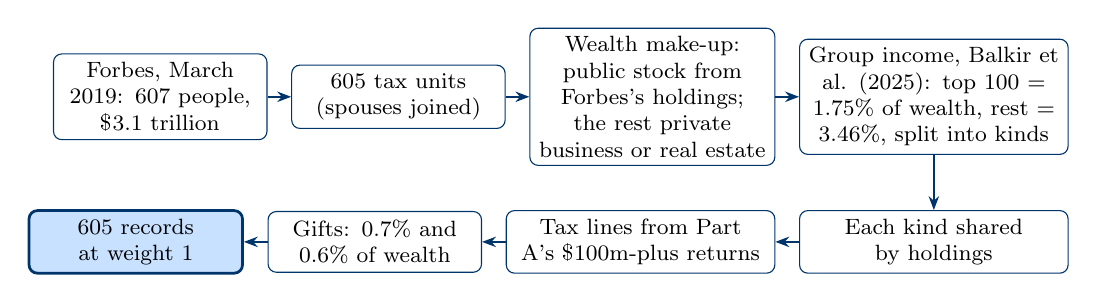
\begin{tikzpicture}[node distance=0.3cm]
    \node[sm, text width=2.5cm] (b1) {Forbes, March 2019: 607 people, \$3.1 trillion};
    \node[sm, text width=2.5cm, right=of b1] (b2) {605 tax units (spouses joined)};
    \node[sm, text width=2.9cm, right=of b2] (b3) {Wealth make-up: public stock from Forbes's holdings; the rest private business or real estate};
    \node[sm, text width=3.2cm, right=of b3] (b4) {Group income, Balkir et al. (2025): top 100 = 1.75\% of wealth, rest = 3.46\%, split into kinds};
    \draw[arr] (b1)--(b2); \draw[arr] (b2)--(b3); \draw[arr] (b3)--(b4);
    \node[sm, text width=3.2cm, below=0.7cm of b4] (b5) {Each kind shared by holdings};
    \node[sm, text width=3.2cm, left=of b5] (b6) {Tax lines from Part A's \$100m-plus returns};
    \node[sm, text width=2.5cm, left=of b6] (b7) {Gifts: 0.7\% and 0.6\% of wealth};
    \node[sm, text width=2.5cm, left=of b7, fill=yalelight!35, line width=1pt] (b8) {605 records at weight 1};
    \draw[arr] (b4)--(b5); \draw[arr] (b5)--(b6); \draw[arr] (b6)--(b7); \draw[arr] (b7)--(b8);
  \end{tikzpicture}

  \vspace{0.8em}
  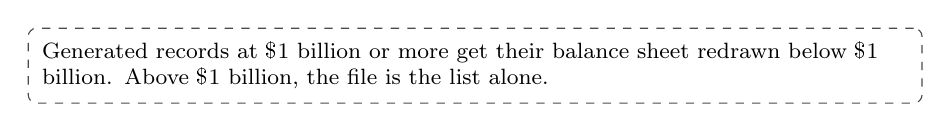
\begin{tikzpicture}
    \node[note, text width=11cm] {Generated records at \$1 billion or more get their balance sheet redrawn
      below \$1 billion. Above \$1 billion, the file is the list alone.};
  \end{tikzpicture}
\end{frame}

% 8
\begin{frame}{Part B: a worked example}
  \small
  Illustrative numbers.
  \begin{enumerate}
    \item The top group's wealth is \$1,000 billion. Its dividends total
          1,000 $\times$ 1.75\% $\times$ 28\% = \$4.9 billion.
    \item Dividends are shared in proportion to public stock.
    \item Zuckerberg holds 15\% of the group's public stock, so his dividends are
          15\% $\times$ \$4.9 billion = \$0.74 billion.
  \end{enumerate}
\end{frame}

% 9
\begin{frame}{Part C: one reweighting}
  \centering
  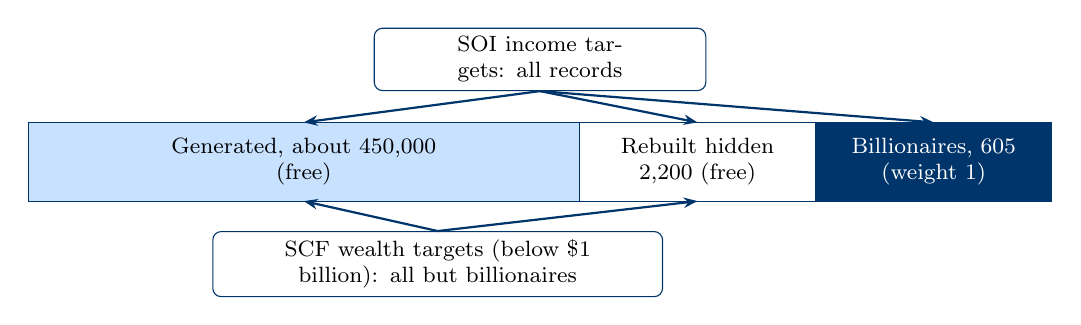
\begin{tikzpicture}
    \draw[draw=yaleblue, fill=yalelight!35] (0,0) rectangle (7,1);
    \draw[draw=yaleblue, fill=white] (7,0) rectangle (10,1);
    \draw[draw=yaleblue, fill=yaleblue] (10,0) rectangle (13,1);
    \node[font=\footnotesize, align=center] at (3.5,0.5) {Generated, about 450,000\\(free)};
    \node[font=\footnotesize, align=center] at (8.5,0.5) {Rebuilt hidden\\2,200 (free)};
    \node[font=\footnotesize, white, align=center] at (11.5,0.5) {Billionaires, 605\\(weight 1)};
    \node[sm, text width=4cm] (t1) at (6.5,1.8) {SOI income targets: all records};
    \draw[arr] (t1.south) -- (3.5,1);
    \draw[arr] (t1.south) -- (8.5,1);
    \draw[arr] (t1.south) -- (11.5,1);
    \node[sm, text width=5.5cm] (t2) at (5.2,-0.8) {SCF wealth targets (below \$1 billion): all but billionaires};
    \draw[arr] (t2.north) -- (3.5,0);
    \draw[arr] (t2.north) -- (8.5,0);
  \end{tikzpicture}

  \vspace{1.0em}
  \footnotesize
  \begin{minipage}{0.9\textwidth}
  \begin{itemize}
    \item Example: the top 0.001\% AGI target is \$214.5 billion. The billionaires contribute a fixed
          \$60 billion (illustrative), so the free records supply \$154.5 billion.
    \item No double count: SOI's totals include the billionaires, whose share is subtracted; the SCF wealth targets stop at \$1 billion.
    \item A check before solving stops the run if any target is out of reach.
  \end{itemize}
  \end{minipage}
\end{frame}

% 10
\begin{frame}{Results}
  \small
  \begin{itemize}
    \item 2015: top 0.001\% AGI is \$216 billion, against SOI's \$215 billion. Without the rebuilt
          returns it is \$103 billion.
    \item 2019: all 805 targets are met. Top 0.001\% AGI is \$212.3 billion, against SOI's \$214.5 billion.
    \item Billionaire AGI per unit, top group: \$329 million, against \$345 million in the IRS study.
    \item Gifts per unit, top group: \$133 million, against \$140 million.
    \item The rebuilt over-\$100-million returns fall from \$151 billion to \$65 billion of AGI to make room.
    \item Effective sample of the free records is unchanged at 80.3\%.
  \end{itemize}
  \par\vfill{\scriptsize\color{yalegrey}Nominal dollars of 2015 and 2019 as labelled. Tested on the
    28--29 October networks.}
\end{frame}

% 11
\begin{frame}{Limits}
  \small
  \begin{itemize}
    \item A family fortune is kept as one record.
    \item Income ratios below Forbes rank 400 are extrapolated.
    \item The mix of items inside the hidden groups comes from the network. It is not observed.
    \item Replacing the SCF's households above \$1 billion with the list is an assumption.
    \item The tax calculator has not yet been run on the billionaire records.
  \end{itemize}
\end{frame}

\end{document}
